\chapter{Methodology}
The CAK and FLD equations described in the introduction are, except for in a few theoretical examples, not to be solved analytically. Instead, they are solved using advanced computer codes. This chapter aims to describe how RHD equations are being solved in a computer code. The code at hand is \texttt{mpi-AMRVAC} which, except for optically thin radiative cooling, had until now not included any radiation effects. Additions made during this thesis are a novelty for the code and can in the future be used in the simulations of a multitude of astrophysical situations.

\section{mpi-amrvac} \label{section: methods amrvac}
Modelling of the winds and atmospheres in this thesis is done in \texttt{mpi-AMRVAC} (Message Passing Interface - Adaptive Mesh Refinement Versatile Advection Code) \citep{Porth2014}, a multidimensional, adaptive mesh (magneto-)hydrodynamics code. In the code, several explicit solvers can be used to solve the conservative hydrodynamical equations (\eqref{hd_rho}, \eqref{hd_mom} and \eqref{hd_e}) with source terms defined by the user. An advantage of working with this particular code is that it is developed in house at the centre for mathematical plasma astrophysics (cmpa), which made a close collaboration with the developers possible.\\
To run the code, several scripts are provided:

\begin{itemize}
\item \textbf{Source code:} The source code consists of all the algorithms to solve the equations, apply boundary conditions, refine the mesh, read input and write output, etc... Inside the source code reside several physics modules, e.g. a module for gravity, dust, radiative cooling and viscosity.\\

\item \textbf{user module:} In the user module, the user defines the initial conditions. Also, this is the place to add additional subroutines for user defined source terms, boundary conditions, time-step calculations and extra output variables among others. The subroutines in this file are automatically called by the source code.\\

\item \textbf{parameter file:} The parameter file is where the computational parameters are defined: grid size and resolution, simulation time, which numerical schemes to use, what type of boundary conditions and how many output files the user wants are only a few to be named. This file is consists of a set of parameters and logicals serving as a control panel for the user.\\
\end{itemize}

In the following sections the integration of CAK-theory and FLD in \texttt{mpi-AMRVAC} will be explained, but first a very brief introduction to numerical HD.


\section{HD in mpi-AMRVAC}
\texttt{MPI-AMRVAC} Solves systems of hyperbolic PDE's, for example the HD-equations \eqref{eq: hd_rho}, \eqref{eq: hd_mom} and \eqref{eq: hd_e}. To solve them, the code makes use of a finite volume approach. In this section, the basic ideas of this approach are explained. Remember the shape of the HD equations in their conservative form, in one dimension they look like:
\begin{align}
\partial_t u + \partial_x f_u &= S_u \label{eq: cons form}
\end{align}
where $u$ is the conserved quantity and $F_u$ is its relevant flux. $S_u$ is the source term, which for the sake of simplicity is put to zero in this explanation. In earlier more primitive methods this equation would be discretized by writing down the derivatives in a discrete way at each cell center. A finite volume method on the other hand treats the value of $u$ as an average over a small volume instead of as a value at a single point. The flux $F_u$ is a quantity existing at the cell faces. Discretization for a finite volume method thus begins by taking the average of $u$ in a finite volume cell by means of integration:
\begin{align} 
\int_{t^n}^{t^{n+1}} \int_{x_{i-\frac{1}{2}}}^{x_{i+\frac{1}{2}}} \left( \partial_t u + \partial_x f_u \right) dt dx &= 0  \label{eq: fin_vol_int}
\end{align}
Define $U$ as the space averaged value for $u$, and $F$ as the time averaged value for $f_u$, the above equation \ref{eq: fin_vol_int} can be written as:
\begin{align}
U^{n+1}_i = U^n_i - \frac{\Delta t}{\Delta x}\left(F^n_{i+\frac{1}{2}} - F^n_{i-\frac{1}{2}} \right) 
\end{align}
A good solver will give an accurate yet computationally cheap expression for the time integrated fluxes$F^n_{i+\frac{1}{2}}$ and $F^n_{i-\frac{1}{2}}$, which are not known analytically. Estimating the values of $F$ is done by a \emph{Riemann solver}. \texttt{MPI-AMRVAC} has a few of these Riemann solvers, including  hll, hllc, roe, tvdlf, etc.. \citep{Toth1996}. The approximations for $F^n_{i+\frac{1}{2}}$ will depend on $u$ and $f_u$.\\ 

\section{CAK-theory}
CAK-theory describes a line driving force and thus an acceleration $g_{CAK}$. This acceleration, together with electron scattering acceleration $g_e$ and gravity $g_{grav}$, enter the  HD momentum equation as source terms. The momentum source terms are added in the user module which is called from the source code. The simulations in this thesis are done in a 1D numerical domain and the radiative force are pointed radially outward. All parameters are defined, and $dv/dr$ is calculated using a centred finite difference:
\begin{align}
S_{\rho \vec{v},i,j} = \rho_{i,j} \frac{1}{1-\alpha} \frac{\kappa_e L_* \bar{Q}}{4\pi r_{i,j}^2 c} \left( \frac{1}{\rho_{i,j} c \bar{Q} \kappa_e} \right)^\alpha \frac{v_{i+1} - v_{i-1}}{r_{i+1} - r_{i-1}}
\end{align}
where $r$ is the radial coordinate. Because of the extra source terms, it is critical to adjust the numerical time step. One doesn't want matter to be accelerated over the length of multiple cells in one time step. In the gravity module for \texttt{MPI-AMRVAC}, the timestep is taken to be the minimum of the hydrodynamical time step calculated on the basis of the characteristic speeds (see section \ref{section: m: FLD}) and the time it takes for an gas element to be accelerated the distance of one numerical cel $\Delta x$:
\begin{align}
dt = \min\left(dt_{HD},\sqrt{\frac{\Delta x}{g_{grav}}} \right)
\end{align}
A similar reasoning is used in the CAK-routine, only now not only $g_{grav}$ but also $g_e$ and $g_{CAK}$ are taken into account.
\begin{align}
dt = \min\left(dt_{HD},\sqrt{\frac{\Delta x}{g_{grav}}},\sqrt{\frac{\Delta x}{g_{e}}},\sqrt{\frac{\Delta x}{g_{CAK}}} \right)
\end{align}
When modelling stellar winds, it is important to also take into account a gravitational acceleration $g_{grav} = \frac{GM}{r^2}$ in the opposite direction. This term is calculated in the user module as well.\\
In the CAK models done in this thesis, the stellar winds where assumed to be isothermal. The isothermal gas assumption is made by switching off the solving for the energy equation in the parameter file. The code now neglects equations \eqref{eq: hd_e} and \eqref{eq: gas_closing}, and replaces them with a new closure relation:
\begin{align}
 p &= a_{adiab} p^\gamma
\end{align}
The two parameters $a_{adiab}$ and $\gamma$ are set to .... and .... to match the conditions in a typical CAK wind for hot massive stars. \citep{Owocki2013}\\


\section{Flux Limited Diffusion} \label{section: m: FLD}
Solving the radiation hydrodynamics equations with an FLD approximation is more complicated than only adding the radiation force as in CAK-theory. For CAK, only the continuity and momentum equations where solved in only one dimension and a sourceterm was added to the momentum equation. For FLD, an entirely new equation has to be solved, source terms need to be added to this new equation, source terms need to be added to the momentum and gas energy equations, and a bunch of new variables, parameters and subroutines have to be defined, designed and written. Given the complexity of the problem, it is solved in a new physics module in the source code. The module will first be worked out for a Cartesian, 2D-case. Lets have a closer look at the additions to the code \\

Continuity equation \eqref{eq: rhd_rho} is as it is and doesn't need any sourceterms.
\begin{align}
S_{\rho} = 0
\end{align}
Momentum equation \eqref{eq: rhd_mom} needs a source term equivalent to the radiation force, which can be computed with the help of the FLD closure relation \eqref{eq: fld_closing}:
\begin{align}
S_{\rho \vec{v}} = \frac{\rho \kappa F}{c}
\end{align}

The radiative energy is added to the code as a variable and evolved trough time. Every time step, the radiative flux is computed from this radiative energy density. $S_{\rho \vec{v}}$ Is added to the momentum field every time step.\\

The gas energy equation needs two source terms, the radiation heating and the radiation cooling:
\begin{align}
S_{e} = -4\pi \kappa \rho B + c \kappa \rho E 
\end{align}

The source terms in the gas energy equation \eqref{eq: hd_e} depend on $E$ and evolve on a radiation timescale instead of a hydrodynamical timescale. For this reason they will be implemented with an implicit scheme, see section \ref{subsection: BIS}.\\

To strengthen this argument, lets give some order of magnitude estimate of the two timescales on which the gas dynamics and the radiation dynamics change. The hydrodynamical timescale can be estimated by the time it takes for a sound wave, travelling at the speed of sound $a_s$, to cross one scale height $H_{eff}$. On the other hand, the radiation timescale is the time it takes a photon to travel the photon mean free path $l_\gamma$ at lightspeed $c$.

\begin{align}
\tau_{HD} &= \frac{H_{eff}}{a_s}= \frac{a_s}{(1-\Gamma)g} \\
\tau_{rad} &= \frac{l_\gamma}{c} = \frac{1}{\kappa \rho c}
\end{align}
After plugging in the typical values for a stellar atmosphere surrounding a $150 M_\odot$ star ($a_s \sim 10^6 \frac{m}{s}$, $\Gamma \sim 0.5$, $g \sim 10^3 \frac{m}{s^2}$, $\kappa \sim 0.34 \frac{cm^2}{g}$ and $\rho \sim 10^{-8}$), we get the following orders of magnitude for the timescales: $\tau_{HD} \sim 10^{3}$ and $\tau_{rad} \sim 10^{-2} $, which is a 5 magnitude difference. Thus:
\begin{align}
\tau_{rad} << \tau_{HD}
\end{align} 

The radiation energy equation \eqref{eq: RHD_op_splt} is entirely new to the code, and the same timescale argument can be applied here. A partially implicit method will be used for solving this equation, in an operator split manner: \\

\begin{align}
\partial_t \left(E \right) + \underbrace{\vec{\nabla} \cdot \left( \vec{v} E \right)}_{1}  &= - \underbrace{\vec{\nabla} \cdot \vec{F}}_{2} - \underbrace{\vec{\nabla} \cdot \vec{v} P + 4\pi \kappa\rho B - c \kappa \rho E}_{3} \label{eq: RHD_op_splt}\\
\end{align} 

\begin{itemize}
\item \textbf{1: The advection term}
\begin{equation}
\partial_t E + \vec{\nabla} \cdot \left( \vec{v} E \right) = 0
\end{equation}
can be handled using already existing \texttt{mpi-AMRVAC} routines, this part has a similar shape to the conservative form of the HD equations \eqref{eq: cons form}. This advection is the movement of the radiation field with the gas, it's a process evolving on a similar timescale as the advection of other quantities. Implementation is as simple as defining the fluxes $f$ and calling the necessary, already existing, subroutines. The code will use the same Riemann solver as used for the other HD variables.\\

\item \textbf{2: The diffusion term}
\begin{align}
\partial_t E = - \vec{\nabla} \cdot \vec{F}
\end{align}
can, by using the FLD closing relation equation \ref{eq: fld_closing}, be written as:
\begin{align}
\partial_t E = - \vec{\nabla} \cdot \left( -\frac{\lambda c}{\kappa \rho} \nabla E\right)
\end{align}
Trying to solve this equation together with the other hydro equations gives rise to two problems. First: the timescale on which the radiation energy $E$ evolves is much shorter than the hydrodynamical timescale on which $\rho$, $\vec{v}$ and $e$ evolve, and second: this is a hyperbolic equation, which makes it hard to solve with the explicit schemes which are used by \texttt{MPI-AMRVAC} to solve the other equations. A way to overcome these problems is solving for the diffusion implicitly. The technique used in developing the new physics module is an Alternative Direction Implicit scheme (ADI), and is based on \citep{Turner12001}.\\

\item \textbf{3: The photon tiring and the radiation heating and cooling sourceterms}
\begin{align}
\partial_t E = - \vec{\nabla} \cdot \vec{v} P + 4\pi \kappa\rho B - c \kappa \rho E
\end{align}
are also evolving on the faster timescale, hence they must be solved implicitly. This is done with an implicit bisection scheme similar to the technique found in \citep{Turner12001}, which will be explained below.
\end{itemize}

In \texttt{MPI-AMRVAC}, the time step at which to evolve the primitive variables is computed based on the characteristic velocities in the system. These are obtained by computing the eigenvalues of the Jacobian flux matrix $A_{i,j} = \frac{\partial F_i}{\partial u_j}$, where $F_i$ and $u_j$ are the fluxes and conserved quantities in the conservative equations \eqref{eq: conservative}. For HD, these eigenvalues are $c_{adiab} + v$, $c_{adiab}$ and $c_{adiab} - v$, where $c_{adiab} = \sqrt{\gamma\frac{p_{gas}}{\rho}}$ is the adiabatic soundspeed. During computations, waves must not travel across cells, thus the time step should be smaller then the time it takes for an acoustic wave with velocity $c_{adiab} + v$ to travel a distance $\Delta x$ which is the width of one numerical cell.\\

In RHD environments there is an extra type of waves, namely radiation acoustic waves \citep{Mihalas1984a} which can, depending on the ratio between the gas and radiation pressure, travel faster than the sound speed. The time step in the RHD calculations will be calculated as a function of $\sqrt{\gamma\frac{p_{gas} + P_{rad}}{\rho}}$ instead of $\sqrt{\gamma\frac{p_{gas}}{\rho}}$.
\begin{align}
dt = \min \left(\frac{\Delta x}{v + \sqrt{\gamma\frac{p_{gas} + P_{rad}}{\rho}}} \right)
\end{align}
This is the maximum time step at which the advection should be calculated to be numerically viable. The diffusion of the radiation energy field on the other hand will generally happen much quicker, depending on the gradient of the $E$-field and diffusion coefficient. This problem is circumvented by using an implicit scheme, described in section \ref{section: m: ADI}

\subsection{Elliptic vs Hyperbolic}
\subsection{Alternating Direction Implicit Scheme} \label{section: m: ADI}
The diffusion part of the radiative energy equation will be solved using the Alternating Direction Implicit (ADI) scheme. This is a numerical scheme which solves the equation implicitly in the first spatial direction an explicitly in the second for half a time step, and then implicitly in the second spatial direction and explicitly in the first for another half time step. ADI is computationally cheaper than a completely implicit scheme, yet it is possible to converge with very big time steps compared to explicit schemes. Lets first simplify the equation by defining the diffusion coefficient $D = \frac{\lambda c}{\kappa \rho}$:
\begin{align}
\partial_t E  = \vec{\nabla} \cdot \left(D \nabla E\right) \label{eq: diffusion}
\end{align}

Lets now construct a numerical scheme. First, the left hand side of \eqref{eq: diffusion} is written in a discrete form. Let $E_{i,j}$ be the radiative energy in cell $(i,j)$ on a grid with $\Delta x$ grid spacing in the $x$-direction and $\Delta y$ grid spacing in the $y$-direction. $D_{i,j}$ is the cell centred diffusion coefficient, whilst $D1_{i,j} = \frac{1}{2} (D_{i+1,j} + D_{i,j})$ and $D2_{i,j} = \frac{1}{2} (D_{i,j+1} + D_{i,j})$ are the cell faced values. To transform from cell center to cell face it is simplest to take the mean of the two surrounding cells. Taking the mean of the six surrounding cells is also an option. 
\begin{align}
\left( \vec{\nabla} \cdot \left(D \nabla E\right) \right)_{i,j} 
 &= \frac{D1_{i+1,j} (\nabla E)_{x} - D1_{i,j} (\nabla E)_{x}}{\Delta x} \\
 &+ \frac{D2_{i,j+1} (\nabla E)_{y} - D2_{i,j} (\nabla E)_{y}}{\Delta y} \\ 
 &= \frac{D1_{i+1,j} (E_{i+1,j} - E_{i,j}) - D1_{i,j} (E_{i,j} - E_{i-1,j})}{\Delta x^2} \\
 &+ \frac{D2_{i,j+1} (E_{i,j+j} - E_{i,j}) - D2_{i,j} (E_{i,j} - E_{i,j-1})}{\Delta y^2} \\ 
\end{align}

For the implicit scheme the diffusion coefficients are chosen at the previous time step, as they are to be computed from a known radiation energy. Evolving \eqref{eq: diffusion} over a time step $\Delta t$ from time $n$ to time $n+1$ then means solving the following equations:
\begin{align}
\frac{E^{n+1} - E^{n}}{\Delta t} = \vec{\nabla} \cdot \left(D^n \nabla E^{n+1}\right) \label{eq: Error_control}
\end{align}

As mentioned before, the ADI scheme first solves half a time step implicitly in for example the $x$-direction and explicitly in the $y$-direction:
\begin{align}
\frac{E_{i,j}^{n+\frac{1}{2}} - E_{i,j}^{n}}{\Delta t}
 &= \frac{D1_{i+1,j}^{n}}{\Delta x^2} (E_{i+1,j}^{n+\frac{1}{2}} - E_{i,j}^{n+\frac{1}{2}}) \\
 &- \frac{D1_{i,j}^{n}}{\Delta x^2} (E_{i,j}^{n+\frac{1}{2}} - E_{i-1,j}^{n+\frac{1}{2}}) \\
 &+ \frac{D2_{i,j+1}^{n}}{\Delta y^2} (E_{i,j+j}^{n} - E_{i,j}^{n}) \\
 &- \frac{D2_{i,j}^{n}}{\Delta y^2} (E_{i,j}^{n} - E_{i,j-1}^{n})
\end{align}
Here it is clear how this step is implicit in the $x$-direction, this expression features the terms $E_{i+1,j}^{n+\frac{1}{2}}$ and $E_{i-1,j}^{n+\frac{1}{2}}$. Yet it is implicit in $y$, there are no $E_{i,j+1}^{n+\frac{1}{2}}$ or $E_{i,j-1}^{n+\frac{1}{2}}$ terms. This is portrayed in Fig. \ref{fig: ADI_stencil}.\\
\begin{figure}
\centering	
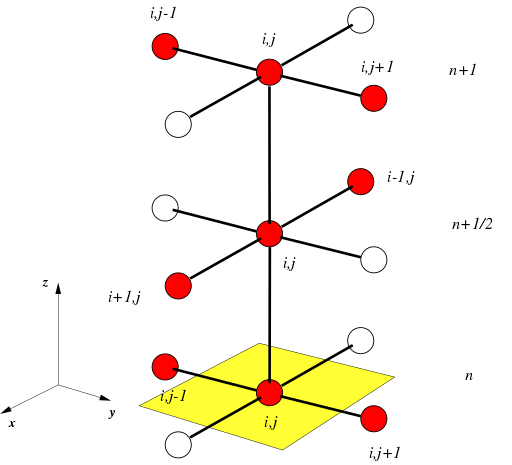
\includegraphics[scale=0.5]{ADI-stencil.png}
\label{fig: ADI_stencil}
\caption{This stencil portraits the working of the ADI scheme, the first half time step from $t=n$ to $t = n +\frac{1}{2}$ depends implicitly on the cells with coordinates $(i+1,j)$, $(i,j)$ and $(i-1,j)$. The second half time step to $t = n+1$ depends implicitly on cells $(i,j+1)$, $(i,j)$ and $(i,j-1)$. Courtesy: wikipedia.}
\end{figure}

In a more simple form, this can be written as:
\begin{align}
\left(1 + \frac{\Delta t D1_{i+1,j}^{n}}{\Delta x^2} + \frac{\Delta t D1_{i,j}^{n}}{\Delta x^2} \right) E_{i,j}^{n+\frac{1}{2}} - \frac{\Delta t D1_{i+1,j}^{n}}{\Delta x^2} E_{i+1,j}^{n+\frac{1}{2}} - \frac{\Delta t D1_{i,j}^{n}}{\Delta x^2} E_{i-1,j}^{n+\frac{1}{2}} = b_{i,j}
\end{align}
where $b_{i,j} = \left(1 + \frac{\Delta t D2_{i,j+1}^{n}}{\Delta y^2} + \frac{\Delta t D2_{i,j}^{n}}{\Delta y^2}\right) E_{i,j}^{n} + \frac{\Delta t D2_{i,j+1}^{n}}{\Delta y^2} E_{i,j+1}^{n} + \frac{\Delta t D2_{i,j}^{n}}{\Delta y^2} E_{i,j-1}^{n}$
Or in matrix form:
\begin{align}
&\begin{bmatrix}
\ddots & \ddots & & &\\
\ddots & \left(1 + \frac{\Delta t D1_{i,j}^{n}}{\Delta x^2} + \frac{\Delta t D1_{i-1,j}^{n}}{\Delta x^2} \right) & -\frac{\Delta t D1_{i,j}^{n}}{\Delta x^2} & & \\
& -\frac{\Delta t D1_{i,j}^{n}}{\Delta x^2} & \left(1 + \frac{\Delta t D1_{i+1,j}^{n}}{\Delta x^2} + \frac{\Delta t D1_{i,j}^{n}}{\Delta x^2} \right) & - \frac{\Delta t D1_{i,j}^{n}}{\Delta x^2} & \\
& & -\frac{\Delta t D1_{i+1,j}^{n}}{\Delta x^2} & \left(1 + \frac{\Delta t D1_{i+2,j}^{n}}{\Delta x^2} + \frac{\Delta t D1_{i+1,j}^{n}}{\Delta x^2} \right) & \ddots \\
& & & \ddots & \ddots
\end{bmatrix} \\
&\times
\begin{bmatrix}
           \vdots                    \\
           E_{i-1,j}^{n+\frac{1}{2}} \\
           E_{i,j}^{n+\frac{1}{2}}   \\
           E_{i+1,j}^{n+\frac{1}{2}} \\
           \vdots
\end{bmatrix} 
=
\begin{bmatrix}
           \cdots & b_{i,j-1} & b_{i,j} & b_{i,j+1} & \cdots
\end{bmatrix}
\end{align}
This is, depending on boundary conditions, a tridiagonal matrix. In \texttt{MPI-AMRVAC}, this matrix system is solved on the entire computational domain and the innermost layer of ghost cells. The boundary conditions on the radiation energy field are applied after the halved time step. This way, the matrix can be kept tridiagonal independent of those boundary conditions. The tridiagonal system is then solved using Thomas' algorithm, which is a simplified form of Gaussian elimination. If the computational grid is $N$ cells by $M$ cells this is an $(N+2) \times (N+2)$ system, and there are $M+2$ such systems to be solved to evolve half a time step. \\

The second half of the time step will be solved implicitly in the $y$-direction and explicitly in $x$-direction. Notice again the diffusion coefficient can only be updated at the end of the cycle:
\begin{align}
\frac{E_{i,j}^{n+1} - E_{i,j}^{n+\frac{1}{2}}}{\Delta t}
 &= \frac{D1_{i+1,j}^{n}}{\Delta x^2} (E_{i+1,j}^{n+\frac{1}{2}} - E_{i,j}^{n+\frac{1}{2}}) \\
 &- \frac{D1_{i,j}^{n}}{\Delta x^2} (E_{i,j}^{n+\frac{1}{2}} - E_{i-1,j}^{n+\frac{1}{2}}) \\
 &+ \frac{D2_{i,j+1}^{n}}{\Delta y^2} (E_{i,j+j}^{n+1} - E_{i,j}^{n+1}) \\
 &- \frac{D2_{i,j}^{n}}{\Delta y^2} (E_{i,j}^{n+1} - E_{i,j-1}^{n+1})
\end{align}
And this system, of course, has a matrix notation completely analogous to the one in the first half of the time step, which can be solved in an analogous way. This time there are $N+2$ matrices of size $(M+2) \times (M+2)$ to be solved. \\

The accuracy of this scheme can be checked by computing and comparing both the left hand side (LHS) and right hand side (RHS) of equation \eqref{eq: Error_control} after calculating $E^{n+1}$. The error is defined by taking the maximum value of the difference of the LHS and RHS weighted with the ratio of the radiative energy and the hydrodynamical time step \citep{Turner12001}:
\begin{align}
Error = \max_{i,j} \left(\frac{\frac{E^{n+1} - E^{n}}{\Delta t} -  \vec{\nabla} \cdot \left(D \nabla E\right)}{E^{n}/dt} \right) \label{eq: Error}
\end{align}

In a completely correct computation, the left hand side would correspond exactly to the right hand side, however due to numerical computations and assumptions this will almost never truly hold.\\

 Test calculations show that this error is often rather large, depending on the distribution of the radiation and density field in the simulation space. A solution is given in \citep{Turner12001} by means of pseudo-time stepping. This method will be explained in the next section.
 
 
\subsection{Pseudo-Time Stepping}
Instead of solving equation \eqref{eq: diffusion} a new variable is introduced, the \emph{pseudotimestep} $w$. The ADI-method is used to solve 
\begin{align}
\partial_w E = \partial_t E  - \vec{\nabla} \cdot \left(D \nabla E\right)
\end{align}
which reduces to \eqref{eq: diffusion} when $\partial_w E = 0$. The pseudo-time step $\Delta w$ can be adjusted independently from the hydrodynamical time step and is increasing in size to converge toward a $w$-stationary state where $\partial_w E = 0$ \citep{Turner12001}.\\

The implicit scheme to evolve half a pseudo-time step from $m$ to $m + \frac{1}{2}$, implicit in the $x$-direction, looks like:
\begin{align}
\frac{E_{i,j}^{m+\frac{1}{2}} - E_{i,j}^{m}}{\Delta w} 
 &= \frac{E_{i,j}^{m+\frac{1}{2}} - E_{i,j}^{n}}{\Delta t} \\
 &- \frac{D1_{i+1,j}^{n}}{\Delta x^2} (E_{i+1,j}^{m+\frac{1}{2}} - E_{i,j}^{m+\frac{1}{2}}) \\
 &+ \frac{D1_{i,j}^{n}}{\Delta x^2} (E_{i,j}^{m+\frac{1}{2}} - E_{i-1,j}^{m+\frac{1}{2}}) \\
 &- \frac{D2_{i,j+1}^{n}}{\Delta y^2} (E_{i,j+j}^{m} - E_{i,j}^{m}) \\
 &+ \frac{D2_{i,j}^{n}}{\Delta y^2} (E_{i,j}^{m} - E_{i,j-1}^{m})
\end{align}

where, again, the diffusion coefficient is considered constant throughout the full hydrodynamical time step. This corresponds to a similar tridiagonal matrix equation which has to be solved for every pseudo-time step. Following, the size of the pseudo-time step $\Delta w$ is exponentially increasing in size per iteration $m = 1 ... W$ and is given by:
\begin{align}
\Delta w = \Delta w_0 \left(\frac{\Delta w_1}{\Delta w_0} \right)^\frac{m-1}{W-1}
\end{align}

$\Delta w_0$ And $\Delta w_1$ are one quarter of the size of a grid cell and one quarter of the size of the numerical domain, respectively. The error of this combined ADI-pseudo-time step method is measured after $W$ pseudo-time steps using \eqref{eq: Error}, if it is too large, $W$ and $\Delta w_1$ are increased whilst $\Delta w_0$ is decreased. If it still doesn't suffice, the above scheme can be applied twice to half a hydrodynamical time step, four times to a quarter hydrodynamical time step, etc. In the testcases described in section \ref{section: res: diff_test}, typically ...4... pseudo-time teps where necessary to reach convergence, depending on the hydro time step.

\subsection{Bisection Implicit Scheme} \label{subsection: BIS}
Solving for the source terms in the gas and radiation energy equations is carried out with another implicit scheme. 
\begin{align}
e^{n+1} - e^n &= \Delta t \left( -4\kappa \sigma \left(\frac{(\gamma - 1)e^{n+1}}{\rho}\right)^4 + c \kappa E^{n+1} \right) \\ 
E^{n+1} - E^n &= \Delta t \left( +4\kappa \sigma \left(\frac{(\gamma - 1)e^{n+1}}{\rho}\right)^4 - c \kappa E^{n+1} -\nabla \vec{v} P^{n+1} \right)
\end{align} 
This can be rewritten as:
\begin{align}
e^{n+1} - e^n &= -a_1 \left( e^{n+1}\right)^4 + a_2 E^{n+1}  \\ 
E^{n+1} - E^n &= a_1 \left( e^{n+1} \right)^4 - a_2 E^{n+1} - a_3 E^{n+1} 
\end{align}
where $a_1 = 4\kappa \sigma \left(\frac{(\gamma - 1)}{\rho^{n+1}}\right)^4 \Delta t$, $a_2 = c \kappa \Delta t$ and $a_3 = \frac{\nabla \vec{v} P^{n+1} }{E^{n+1}} \Delta t$. Manipulation of the equations returns:
\begin{align}
E^{n+1} &= \frac{a_1 \left( e^{n+1} \right)^4 + E^n}{1 + a_2 + a_3} \label{eq: E_src}
\end{align}
And
\begin{align}
\left( e^{n+1} \right)^4 &+ \frac{1 + a_2 + a_3}{a_1 + a_3}e^{n+1} -  \frac{(1 + a_2 + a_3)e^n + a_2 E^n}{a_1 + a_3} = 0 \label{eq: Poly}
\end{align}

Equation \eqref{eq: Poly} is a $4^{th}$ degree polynomial in $e^{n+1}$, with a single root between $0$ and $\frac{1 + a_2 + a_3}{a_1 + a_3}$. This is solved for $e^{n+1}$ using the bisection method to calculate the contribution of the radiative heating and cooling to the gas energy. The newly calculated $e^{n+1}$ is then plugged in equation \eqref{eq: E_src} to find the contribution of the radiative heating and cooling, and the photon tiring to the radiation energy.

\section{Dimensionless problem}
Computationally, floating point values are the most precise around unity. For this reason, it is preferable to rescale physical quantities such as $\rho$, $\vec{v}$, $e$, ... with values typical to the simulation domain. \texttt{mpi-AMRVAC} already does part of this for us, in the user module, one can define the units for either number density, temperature  and length ($N_0$, $T_0$, $l_0$) or for number density, velocity  and length ($N_0$, $v_0$, $l_0$). The other units will be then computed from these quantities using the following relations:
\begin{align}
\rho_0 &= \mu m_p N_0 \\
   p_0 &= \gamma N_0 k_b T_0 \\
   v_0 &= \sqrt{\frac{p_0}{\rho_0}} \\
   t_0 &= \frac{l_0}{v_0}
\end{align}
Calculations in \texttt{MPI-AMRVAC} are always done with unit less quantities, in HD these are: $\tilde{\rho} = \frac{\rho}{\rho_0}$, $\tilde{\vec{v}} = \frac{\vec{v}}{\vec{v}_0}$, $\tilde{p} = \frac{p}{p_0}$ and $\tilde{e} = \frac{e}{p_0}$. Using this, we can transform the continuity equation \eqref{eq: hd_rho} to dimensionless units:
\begin{align}
\frac{t_0}{\rho_0} \frac{\partial}{\partial t} \rho  + \frac{t_0}{\rho_0} \vec{\nabla} \cdot \left( \rho \vec{v}  \right) &= \frac{t_0}{\rho_0} S_\rho \\
\frac{\partial}{\partial \tilde{t}} \tilde{\rho} + \tilde{\nabla} \left( \tilde{\vec{v}} \tilde{\rho} \right) &= \tilde{S}_\rho
\end{align}
Where $\nabla$ has the units of reciprocal length and $\tilde{S}_\rho \def \frac{t_0}{\rho_0} S_\rho$. Equivalently, for the momentum equation \eqref{eq: hd_mom} and the gas energy equation \eqref{eq: hd_e}:
\begin{align}
\frac{\partial}{\partial \tilde{t}} \left(\tilde{\rho} \tilde{\vec{v}} \right) + \tilde{\vec{\nabla}} \left(\tilde{\vec{v}} \tilde{\rho}  \tilde{\vec{v}} + \tilde{p} \right) &= \tilde{S}_{\rho \vec{v}} \\
\frac{\partial}{\partial \tilde{t}} \tilde{e} + \tilde{\vec{\nabla}} \left(\tilde{\vec{v}} \tilde{e} + \tilde{\vec{v}} \tilde{p} \right) &= \tilde{S}_e \\
\end{align}
$\tilde{S}_{\rho \vec{v}} = S_{\rho \vec{v}} \frac{t_0}{\rho_0 v_0}$ and $\tilde{S}_e = S_e \frac{t_0}{e_0}$ are the momentum and energy equation source terms. For the RHD equations this will rescale the physical constants:
\begin{align}
	\tilde{S}_{\rho \vec{v}} &=  \frac{\kappa \rho}{c} \vec{F} \frac{t_0}{\rho_0 v_0} \\
							 &=  \frac{\tilde{\kappa}\tilde{\rho}}{\tilde{c}} \tilde{\vec{F}} \\
	\tilde{S}_e &= -4\pi \kappa\rho B \frac{t_0}{e_0}  + c \kappa \rho E \frac{t_0}{e_0} \\
				&= -4 \tilde{\sigma} \tilde{\kappa} \tilde{T}^4 + \tilde{c} \tilde{\rho} \tilde{E}
\end{align}
The rescaled Stefan-Boltzmann constant $\tilde{\sigma}$, the rescaled speed of light $\tilde{c}$ and the rescaled opacity $\tilde{\kappa}$ are given by $\tilde{\sigma} = \frac{\sigma T_0^4}{e_0 v_0}$, $\tilde{c} = \frac{c}{v_0}$ and $\tilde{\kappa} = \kappa v_0 t_0$. The unit of the radiation energy density and radiation flux can also be defined: $E_0 = e_0$ and $F_0 = \rho_0 v_0^3$. These are used to transform the RHD equation for radiation energy \eqref{eq: rhd_e_r} and the FLD closure relation \eqref{eq: fld_closing}. 

\section{Visualisation}
\texttt{mpi-AMRVAC} output is given in binary .vtu files. Special software such as visit \citep{} and paraview are used to open and analyse the simulation results. The standard output consists of the primitive variables at every simulation cell for a specified number of time steps. Extra output variables can be defined in the user module.

